% The CKF depth-first branch walk, and where the Navigator is re-initialised.
% One call to findTracks() is not one trajectory: it is a tree walk, with
% Actor::reset() (CombinatorialKalmanFilter.hpp:471-538) teleporting the stepper
% back and calling navigator.initialize() again, mid-propagation.
\documentclass[border=8pt]{standalone}
\usepackage{tikz}
\usepackage{newtxtext,newtxmath}
\usetikzlibrary{arrows.meta,positioning,calc,decorations.pathreplacing}

\begin{document}
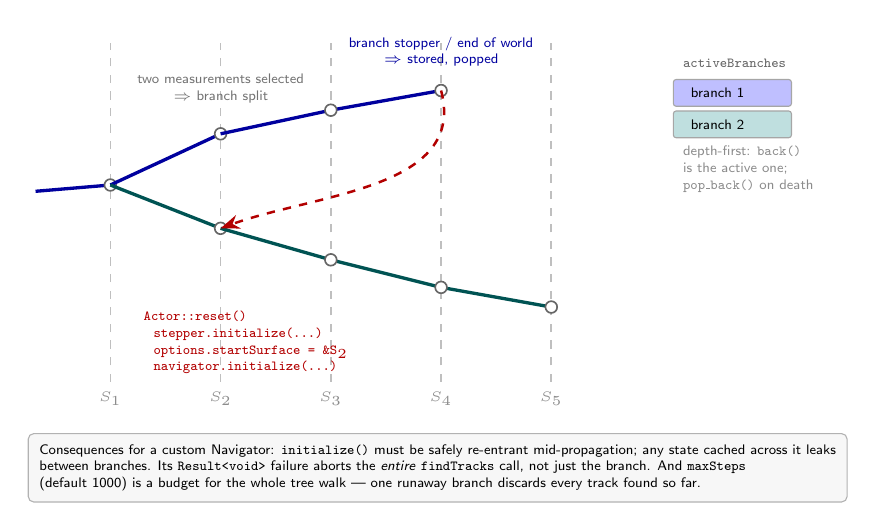
\begin{tikzpicture}[
  scale=1.0,
  font=\sffamily\footnotesize,
  surf/.style={draw=black!25,line width=0.6pt,dashed},
  br/.style={line width=1.2pt,draw=blue!62!black},
  br2/.style={line width=1.2pt,draw=teal!65!black},
  reset/.style={line width=0.9pt,draw=red!70!black,dashed,-{Stealth[length=2.4mm]}},
  st/.style={circle,draw=black!60,fill=white,inner sep=1.5pt,line width=0.6pt},
  lbl/.style={font=\sffamily\scriptsize},
  tny/.style={font=\sffamily\tiny}
]

% ---- surfaces ----
\foreach \x/\n in {1.0/1, 2.4/2, 3.8/3, 5.2/4, 6.6/5} {
  \draw[surf] (\x,-0.4) -- (\x,3.9);
  \node[tny,text=black!45] at (\x,-0.62) {$S_\n$};
}

% ---- root segment ----
\coordinate (a1) at (1.0,2.10);
\draw[br] (0.05,2.02) -- (a1);
\node[st] at (a1) {};

% ---- fork at S2 ----
\coordinate (b1) at (2.4,2.75);
\coordinate (b2) at (2.4,1.55);
\draw[br]  (a1) -- (b1);
\draw[br2] (a1) -- (b2);
\node[st] at (b1) {};
\node[st] at (b2) {};
\node[tny,text=black!55,anchor=south,align=center] at (2.4,3.02)
  {two measurements selected\\ $\Rightarrow$ branch split};

% ---- branch 1 (explored first, then dies) ----
\coordinate (c1) at (3.8,3.05);
\coordinate (d1) at (5.2,3.30);
\draw[br] (b1) -- (c1) -- (d1);
\node[st] at (c1) {};
\node[st] at (d1) {};
\node[tny,text=blue!62!black,anchor=south,align=center] at (5.20,3.48)
  {branch stopper / end of world\\ $\Rightarrow$ stored, popped};

% ---- branch 2 (resumed after reset) ----
\coordinate (c2) at (3.8,1.15);
\coordinate (d2) at (5.2,0.80);
\coordinate (e2) at (6.6,0.55);
\draw[br2] (b2) -- (c2) -- (d2) -- (e2);
\node[st] at (c2) {};
\node[st] at (d2) {};
\node[st] at (e2) {};

% ---- the reset jump ----
\draw[reset] (d1) to[out=-75,in=20] (b2);
\node[tny,text=red!70!black,anchor=north west,align=left] at (1.30,0.62)
  {\texttt{Actor::reset()}\\
   \ \ \texttt{stepper.initialize(...)}\\
   \ \ \texttt{options.startSurface = \&S}$_2$\\
   \ \ \texttt{navigator.initialize(...)}};

% ---- activeBranches stack ----
\begin{scope}[shift={(8.15,0.35)}]
  \node[tny,text=black!60,anchor=west] at (0,3.30) {\texttt{activeBranches}};
  \foreach \i/\y/\c in {0/2.75/blue!25, 1/2.35/teal!25} {
    \draw[draw=black!35,fill=\c,rounded corners=1pt] (0,\y) rectangle ++(1.5,0.34);
  }
  \node[tny,anchor=west] at (0.10,2.92) {branch 1};
  \node[tny,anchor=west] at (0.10,2.52) {branch 2};
  \node[tny,text=black!45,anchor=west,align=left] at (0,1.95)
    {depth-first: \texttt{back()}\\ is the active one;\\ \texttt{pop\_back()} on death};
\end{scope}

% ---- caption ----
\node[draw=black!30,fill=black!3,rounded corners=2pt,inner sep=4pt,
      align=left,tny,anchor=north west] at (-0.05,-1.05)
  {Consequences for a custom Navigator: \texttt{initialize()} must be safely re-entrant mid-propagation;
   any state cached across it leaks\\
   between branches. Its \texttt{Result<void>} failure aborts the \emph{entire} \texttt{findTracks} call,
   not just the branch. And \texttt{maxSteps}\\
   (default 1000) is a budget for the whole tree walk --- one runaway branch discards every track
   found so far.};

\end{tikzpicture}
\end{document}
